\documentclass[conference]{IEEEtran}
\usepackage{graphicx}
\usepackage{cite}
\usepackage{amsmath}
\usepackage{url}
\usepackage{balance}
\usepackage[hidelinks]{hyperref}
\usepackage{booktabs}
\usepackage{listings}
\lstset{
  basicstyle=\footnotesize\ttfamily,
  numbers=left,
  numberstyle=\tiny,
  numbersep=5pt,
  frame=single,
  breaklines=true,
  captionpos=b,
  xleftmargin=2em,
  framexleftmargin=1.5em
}

\begin{document}

\title{Multi-View Visualization of TLA+ State Spaces:\\A Design Study with Coordinated Graph and Matrix Views}

\author{
\IEEEauthorblockN{Anonymous Author(s)}
\IEEEauthorblockA{Anonymous Affiliation\\
Anonymous City, Anonymous Country\\
anonymous@email.com}
}

\maketitle

\begin{abstract}
Mission-critical systems must comply with rigorous formal standards, yet the state spaces produced by model checkers like TLC are difficult for engineers to comprehend. Standard node-link visualizations degenerate into illegible tangles beyond a few dozen states. We present a web-based multi-view visualization tool for TLA+ state spaces that combines a clustered force-directed graph, an adjacency matrix with cluster-based ordering, and a coordinated split view with bidirectional brushing-and-linking. The tool groups states by shared variable values, enabling engineers to understand state structure, verify transitions, and trace execution paths. We describe our design process---including task analysis, data characterization, and design rationale---and demonstrate the tool on three TLA+ specifications of increasing complexity.
\end{abstract}

\begin{IEEEkeywords}
formal methods, TLA+, visualization, state machine, adjacency matrix, coordinated views, design study, model checking
\end{IEEEkeywords}

\section{Introduction}

Formal system specification provides significant advantages for mission-critical systems engineering. Mission-critical systems must comply with rigorous standards---such as DO-178C for airborne software and ISO~26262 for automotive functional safety---that rely heavily on mathematical formalisms to establish correctness. Formal specifications are concise, precise, and amenable to automated verification through model checking and theorem proving. This allows engineers to locate errors in the specification far more precisely---sometimes identifying very challenging faults---than the code of the target system, compared to conventional testing techniques.

Among formal specification languages, TLA+ (Temporal Logic of Actions)~\cite{lamport2003specifying, lamport2009pluscal} has emerged as one of the most widely adopted in industry. TLA+ is a domain-specific language for expressing formal properties of systems based on temporal logic, providing far greater expressiveness and reasoning capability than conventional software design modeling tools. Amazon Web Services uses TLA+ to verify the correctness of complex distributed systems including DynamoDB, S3, and EBS~\cite{newcombe2015amazon}, while Microsoft has applied TLA+ to the development of safety-critical fault-tolerant middleware~\cite{resch2017tla}. The TLC model checker~\cite{yuan1999model} enables engineers to exhaustively enumerate all reachable states and transitions for a given specification, and code developed based on the formal specification is thus far more reliable and errors can be located far earlier and proactively than post-implementation testing techniques.

However, these specifications require deep expertise in temporal logic. For many systems engineers, TLA+ specifications and models are very hard to read and review, limiting the usability of the methods. In most cases, having the right formal methods experts to write specifications does not solve the problem, as the wider development team needs to be able to deeply understand the formal specifications. We want to aid these engineers by applying visualization techniques to translate TLA+ state spaces into intuitive visual representations---such as state machine diagrams, which have been used for decades and are well understood by practitioners and engineers alike~\cite{harel1987statecharts, harel1988visual}. However, the state spaces produced by model checking are inherently difficult to comprehend. Each state in a TLA+ specification represents a complete assignment of values to all specification variables, and each transition corresponds to an action that transforms one state into another. Even for moderately complex specifications, the number of reachable states grows combinatorially with the number of variables and their domains---a phenomenon known as the state explosion problem~\cite{liu2005model}. For example, a specification with ten variables each capable of holding ten distinct values has a theoretical state space of $10^{10}$ states. While the TLC model checker can enumerate these states efficiently, presenting the results to engineers in a comprehensible manner remains an open challenge.

The current state of TLA+ visualization is limited. The TLA+ Toolbox provides textual output from the TLC model checker, listing states and transitions in a sequential format that becomes overwhelming for large specifications. A natural approach to visualizing state spaces is to render them as node-link diagrams using a force-directed layout. However, standard force-directed layouts without clustering or alternative representations degenerate into illegible ``hairball'' diagrams beyond a few dozen states (Fig.~\ref{fig:hairball}). This scalability limitation is well-documented in the graph visualization literature: force-directed layouts produce visual clutter at scale due to edge crossings, node overlaps, and the difficulty of perceiving structure in dense graphs~\cite{harel1988visual, herman2000graph}. Diehl~\cite{diehl2007softvis} provides a comprehensive treatment of software visualization techniques, but existing approaches focus primarily on source code structure and runtime behavior rather than formal specification state spaces.

\begin{figure}[t]
\centering
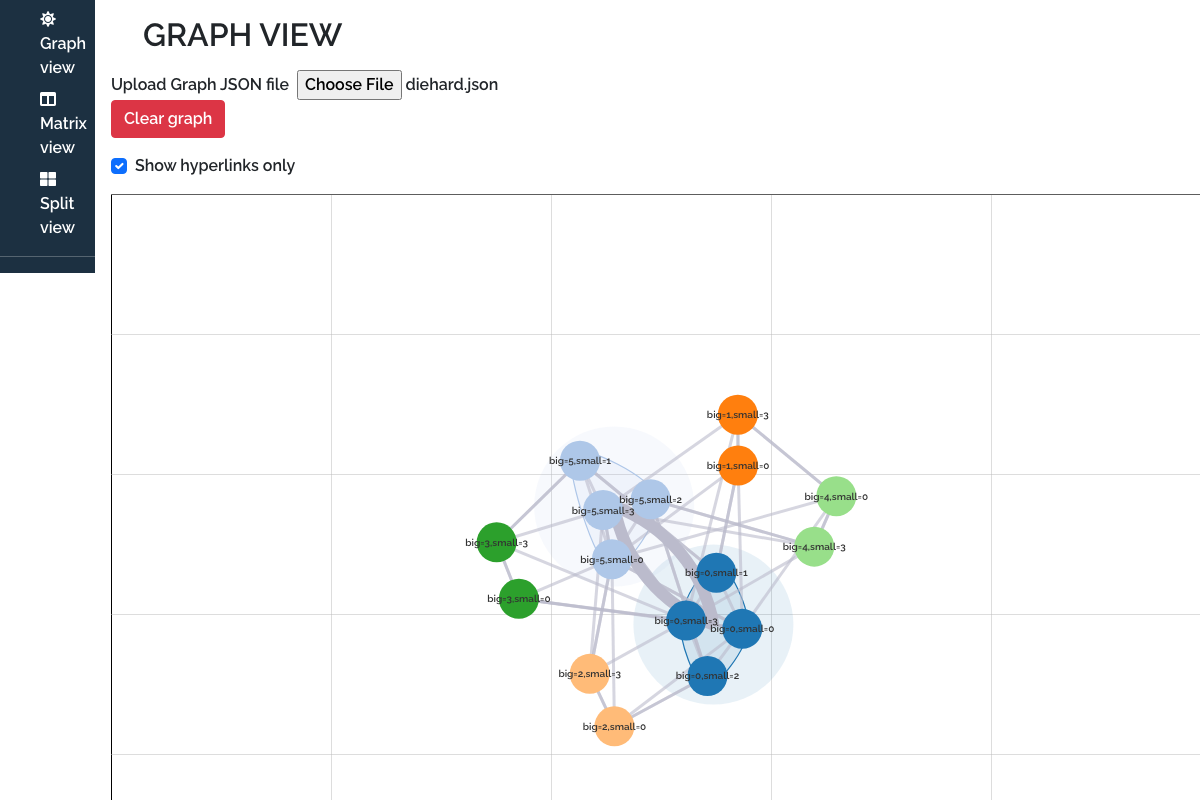
\includegraphics[width=\columnwidth]{figures/diehard_graph.png}
\caption{The Die Hard water jugs specification rendered as a flat force-directed layout without clustering. With 16 nodes and 58 edges, the visualization degenerates into an illegible ``hairball'' where no meaningful structure is visible.}
\label{fig:hairball}
\end{figure}

Research in information visualization has established that different visual representations have complementary strengths for different tasks. Ghoniem et al.~\cite{ghoniem2004comparison} demonstrated through controlled experiments that adjacency matrices outperform node-link diagrams for large, dense graphs on tasks such as finding connections, estimating graph size, and identifying clusters, while node-link diagrams remain superior for path-following tasks. Henry and Fekete~\cite{henry2006matrixexplorer} showed that combining node-link and matrix representations in a coordinated dual-representation system enables users to leverage the strengths of each. The TensorFlow Graph Visualizer~\cite{wongsuphasawat2018tensorflow} further demonstrated that hierarchical clustering, semantic grouping, and interactive detail-on-demand can make computational graphs with thousands of nodes navigable and comprehensible.

Drawing on these insights, we present a design study of a web-based multi-view visualization tool for TLA+ state spaces. Our tool provides three coordinated views: a clustered force-directed graph, an adjacency matrix with cluster-based ordering, and a synchronized split view that links the two representations through a bidirectional highlighting protocol. The design is informed by a task analysis derived from our experience deploying TLA+ specifications in industry projects, a characterization of the data properties of TLC model checker output, and the design rationale documented during our iterative development process.

Following the methodology of visualization design studies~\cite{sedlmair2012design}, we structure our paper around the design process and demonstrate the tool's utility through detailed usage scenarios rather than controlled experiments. This approach is appropriate for a tool paper targeting the intersection of formal methods and visual analytics, where the primary contribution is the design itself and its ability to support real engineering tasks.

We make the following contributions:

\begin{itemize}
\item A \textbf{task analysis} for TLA+ state space visualization, identifying four key tasks that engineers need to perform when examining model checker output.
\item A \textbf{clustered force-directed graph view} that groups states by shared variable values, with convex hull cluster boundaries, color-coded cluster membership, and interactive detail-on-demand through hover-based dimming of non-connected nodes.
\item An \textbf{adjacency matrix view} with cluster-based ordering that reveals connectivity patterns and cluster structure at higher information density than node-link diagrams, supporting reordering by cluster or node identifier.
\item A \textbf{coordinated split view} with bidirectional brushing-and-linking: hovering a state in either view highlights the corresponding state and its connections in the other view, supporting cross-referencing between spatial and structural representations.
\item A \textbf{web-based implementation} using D3.js~\cite{bostock2011d3} that ingests the JSON output of the TLC model checker, requiring no installation beyond a modern web browser.
\item \textbf{Detailed usage scenarios} on three TLA+ specifications of increasing complexity, demonstrating how the multi-view approach supports each identified task.
\end{itemize}

The remainder of this paper is organized as follows. Section~\ref{sec:background} provides background on TLA+ and the TLC model checker. Section~\ref{sec:related} surveys related work in formal methods visualization, graph visualization, matrix-based visualization, and coordinated multiple views. Section~\ref{sec:design} describes our design process, including task analysis, data characterization, and design rationale. Section~\ref{sec:system} presents the design of our visualization tool. Section~\ref{sec:scenarios} demonstrates the tool through detailed usage scenarios. Section~\ref{sec:discussion} discusses our findings, limitations, and future work. Section~\ref{sec:conclusion} concludes the paper.

%% ============================================================
\section{Background: TLA+ and Model Checking}
\label{sec:background}

TLA+ is a formal specification language created by Leslie Lamport for specifying and reasoning about concurrent and distributed systems~\cite{lamport2003specifying}. The language is based on the Temporal Logic of Actions, which combines temporal logic with a theory of actions (state transitions) to describe system behavior. TLA+ specifications describe a system as a state machine: an initial state predicate defines the set of possible starting states, and a next-state relation defines how the system can transition from one state to another. Each state is a complete assignment of values to all specification variables, and each transition is triggered by an action---a named predicate that constrains the relationship between the current state and the next state.

\subsection{A Motivating Example: HourClock}

To illustrate both the power and the comprehension challenge of TLA+ specifications, we use the HourClock example from Lamport's \textit{Specifying Systems}~\cite{lamport2003specifying}. This specification formally describes the behavior of a clock that increments the state variable \texttt{hr} by 1 every iteration until it reaches 12, at which point it cycles back to 1. Fig.~\ref{fig:hourclock_spec} shows the complete TLA+ specification.

\begin{figure}[t]
\begin{lstlisting}[language={},morekeywords={MODULE,EXTENDS,VARIABLE,THEOREM,IF,THEN,ELSE}]
---- MODULE HourClock ----
EXTENDS Naturals
VARIABLE hr
HCini == hr \in (1 .. 12)
HCnxt == hr' = IF hr # 12
                THEN hr + 1
                ELSE 1
HC == HCini /\ [][HCnxt]_hr
THEOREM HC => []HCini
====
\end{lstlisting}
\caption{The HourClock TLA+ specification~\cite{lamport2003specifying}. The variable \texttt{hr} ranges from 1 to 12, and the action \texttt{HCnxt} increments it cyclically.}
\label{fig:hourclock_spec}
\end{figure}

While HourClock is a very simple and basic example of a TLA+ specification, to an untrained eye it is already hard to comprehend: the temporal logic operators (\texttt{[]}, \texttt{[]} with subscript) and the primed variable notation (\texttt{hr'}) are unfamiliar to most software engineers. With larger, more complex system specifications involving multiple variables, guards, and concurrent actions, the difficulty increases dramatically. The system state in this case is just the variable \texttt{hr}, which can take values 1 to 12, producing 12 states connected in a cycle. When the TLC model checker enumerates this state space, it produces a directed graph with 12 nodes and 12 edges---simple enough to visualize, but illustrative of the state machine structure that our tool renders.

\subsection{The TLC Model Checker}

The TLC model checker~\cite{yuan1999model} is the primary verification tool for TLA+ specifications. Given a specification and a set of model constraints (finite domains for each variable), TLC exhaustively enumerates all reachable states and transitions using breadth-first search. The output is a complete state graph $G = (V, E)$ where each vertex $v \in V$ represents a distinct reachable state and each directed edge $(u, v) \in E$ represents a transition from state $u$ to state $v$ triggered by a specific action.

TLC can verify temporal properties (invariants, liveness conditions) during enumeration, reporting counterexamples as traces through the state graph when properties are violated. However, TLC's primary output---the complete state graph---is presented as textual output: a list of states with their variable assignments and a list of transitions between them. For small specifications, this textual output is manageable; for specifications with hundreds or thousands of states, it becomes impractical to read and understand.

\subsection{PlusCal}

PlusCal~\cite{lamport2009pluscal} is an algorithm language that transpiles to TLA+, providing a more familiar imperative syntax for engineers who find temporal logic notation challenging. PlusCal specifications are translated to TLA+ and then verified using TLC. The state spaces produced by PlusCal-derived specifications have the same structure as those produced by hand-written TLA+ specifications, and our visualization tool handles both equivalently.

\subsection{The State Explosion Problem}

A fundamental challenge in model checking is the state explosion problem: the number of reachable states grows combinatorially with the number of specification variables and their domains. Consider a specification with variables $a$, $b$, and $c$ where $a \in \{1, 2, 3, 4\}$, $b \in \{5, 6, 7\}$, and $c \in \{0, 3, 6, 9\}$. The theoretical maximum number of states is $4 \times 3 \times 4 = 48$, though the actual number of reachable states may be smaller depending on the specification's constraints. As the number of variables increases or their domains expand, the state space grows exponentially. A specification with ten variables, each holding ten possible values, has a theoretical state space of $10^{10}$ states---far beyond what any visualization can render directly.

This exponential growth has profound implications for visualization. While TLC can enumerate state spaces with millions of states, presenting even a few hundred states as a flat node-link diagram produces an illegible visualization. Effective visualization of TLA+ state spaces therefore requires techniques that manage complexity through abstraction, clustering, or alternative representations that scale better than standard node-link diagrams.

\subsection{Industry Adoption}

TLA+ has seen significant adoption in industry for verifying critical systems. Newcombe et al.~\cite{newcombe2015amazon} described how Amazon Web Services used TLA+ to find subtle bugs in the designs of DynamoDB, S3, EBS, and an internal distributed lock manager. The specifications helped engineers discover errors that would have been extremely difficult to find through testing alone, and the authors reported that TLA+ had become a standard part of the development process for complex distributed systems at AWS. Resch and Paulitsch~\cite{resch2017tla} documented the use of TLA+ in developing safety-critical fault-tolerant middleware, demonstrating the language's applicability beyond distributed systems to real-time safety-critical domains. These industry deployments motivate the need for better visualization tools: as TLA+ is adopted by engineers who may not have deep expertise in temporal logic, visual representations of state spaces become essential for building understanding and trust in the specifications.

%% ============================================================
\section{Related Work}
\label{sec:related}

Our work draws on four areas of prior research: visualization of formal specifications, graph visualization techniques, matrix-based network visualization, and coordinated multiple views.

\subsection{Formal Methods Visualization and Tooling}

Visualization of formal specifications has received attention across multiple formal methods communities. Harel's Statecharts~\cite{harel1987statecharts} introduced a visual formalism for complex systems based on hierarchical state machines with concurrency, providing a visual notation that has influenced both specification languages and their visualization tools. The Statecharts formalism demonstrated that visual representations of state-based systems can significantly improve comprehension, particularly when hierarchical grouping is used to manage complexity.

For TLA+ specifically, the TLA+ Toolbox provides the TLC model checker with textual output, but does not include graphical visualization of the state space. A straightforward approach is to parse the TLA+ model file, run the TLC model checker to extract states and transitions, and render the result as a force-directed graph. However, a single-view force-directed layout without semantic clustering has limited scalability: for specifications with more than approximately 20 states, the visualization degenerates into a ``hairball'' with overlapping nodes and crossing edges that obscure the structure of the state space (see Fig.~\ref{fig:hairball}).

Other formal methods tools provide visualization capabilities for their respective specification languages. The Alloy Analyzer~\cite{jackson2012alloy} visualizes instances of Alloy specifications as node-link diagrams, with automatic layout and interactive exploration. However, Alloy's visualizer is primarily designed for showing individual instances rather than complete state spaces. ProB~\cite{leuschel2008prob} is an animator and model checker for the B-method~\cite{abrial1996bbook} that provides a graphical state space viewer, but it uses a simple tree layout that does not scale to large state spaces. UPPAAL~\cite{behrmann2004uppaal} provides a graphical editor and simulator for timed automata, with visual representations of automata networks, but focuses on the specification structure rather than the explored state space. The Rodin platform~\cite{abrial2010rodin} for Event-B provides graphical modeling capabilities but limited state space visualization. Liu et al.~\cite{liu2005model} used model checking combined with a replay facility to debug complex distributed systems, demonstrating the value of integrating model checker output with interactive exploration tools.

Across these tools, a common limitation is the reliance on standard node-link diagrams for state space visualization, which inherently limits scalability. Our work addresses this limitation by introducing matrix-based and coordinated multi-view representations that complement the node-link diagram.

\subsection{Graph Visualization Techniques}

Force-directed graph layouts~\cite{harel1988visual} are the most common technique for drawing general graphs. These algorithms model the graph as a physical system where nodes repel each other (like charged particles) and edges act as springs, iteratively moving nodes toward an equilibrium that minimizes edge crossings and distributes nodes evenly. While effective for small graphs, force-directed layouts suffer from several well-documented scalability problems: visual clutter from edge crossings, node overlaps, and the inability to perceive meaningful structure in dense graphs~\cite{herman2000graph}.

Clustered graph visualization addresses some of these problems by grouping related nodes into clusters that are drawn together. Eades et al.~\cite{eades1996hierarchical} formalized the concept of clustered graphs and presented algorithms for drawing them with non-crossing cluster boundaries. Sugiyama et al.~\cite{sugiyama1981hierarchical} introduced hierarchical graph drawing with layered layouts, which has become foundational for drawing directed acyclic graphs. The TensorFlow Graph Visualizer~\cite{wongsuphasawat2018tensorflow} demonstrated that combining hierarchical clustering with edge bundling, interactive expansion, and semantic grouping based on source code namespaces can make dataflow graphs with thousands of nodes navigable. Their approach of using domain-specific metadata (operation names and namespaces) to define the clustering hierarchy is directly analogous to our use of shared variable values to define clusters in TLA+ state spaces.

Dunne and Shneiderman~\cite{dunne2013motif} proposed motif simplification as an approach to reducing visual clutter in node-link diagrams by replacing common network motifs (fans, connectors, cliques) with compact glyphs. While our approach uses clustering rather than motif replacement, the underlying goal---reducing visual complexity while preserving structural information---is the same. Holten~\cite{holten2006hierarchical} introduced hierarchical edge bundling, which routes edges along a hierarchy tree using B-spline curves, dramatically reducing visual clutter in graphs with hierarchical structure. This technique is particularly relevant for clustered state-space graphs where many transitions cross cluster boundaries.

\subsection{Matrix-Based Network Visualization}

Adjacency matrices provide a fundamentally different representation of graphs compared to node-link diagrams. In a matrix representation, rows and columns correspond to nodes, and a filled cell at position $(i, j)$ indicates an edge from node $i$ to node $j$. Bertin~\cite{bertin1983semiology} established the theoretical foundations for matrix-based visualization, demonstrating that reordering rows and columns can reveal patterns such as clusters, blocks, and bands that are invisible in the original ordering. Behrisch et al.~\cite{behrisch2016reordering} provided a comprehensive survey of matrix reordering methods for network visualization, classifying approaches by their optimization criteria and the structural patterns they reveal.

The key advantage of matrix representations for dense graphs is that they avoid edge crossings entirely: every potential connection has a dedicated cell, making it possible to read the connectivity pattern for any node by scanning its row and column. Ghoniem et al.~\cite{ghoniem2004comparison} confirmed this advantage empirically, demonstrating through controlled experiments that adjacency matrices outperform node-link diagrams for large, dense graphs on tasks including finding connections between specific nodes, estimating the number of connections for a node, and identifying clusters. However, they also found that node-link diagrams are superior for path-following tasks, particularly on small, sparse graphs where the spatial layout conveys meaningful information about graph structure.

Henry and Fekete~\cite{henry2006matrixexplorer} introduced MatrixExplorer, a dual-representation system that provides both node-link and matrix views of social networks, allowing users to switch between representations and reorder the matrix interactively. This work demonstrated the practical value of offering multiple representations to users, as each representation reveals different aspects of the network. Henry et al.~\cite{henry2007nodetrix} extended this idea with NodeTrix, a hybrid visualization that embeds adjacency matrices inside the nodes of a node-link diagram: dense communities are shown as compact matrices while inter-community links use traditional edges. Henry and Fekete also introduced MatLink~\cite{henry2007matlink}, which augments adjacency matrices with curved links drawn on the matrix borders to support path-following tasks that matrices traditionally handle poorly. These works collectively establish that combining matrix and node-link representations provides benefits that neither representation achieves alone.

\subsection{Coordinated Multiple Views}

The principle of coordinated multiple views (CMV) is well-established in information visualization. Shneiderman's visual information seeking mantra---``overview first, zoom and filter, then details on demand''~\cite{shneiderman1996eyes}---provides the theoretical basis for interactive exploration of complex data. Roberts~\cite{roberts2007cmv} surveyed the field of coordinated and multiple views, classifying interaction types and coordination mechanisms. North and Shneiderman~\cite{north2000snap} demonstrated through user studies that tight coupling between views through shared data and operations improves user performance in exploratory analysis. Wang Baldonado et al.~\cite{baldonado2000guidelines} established design guidelines for when and how to use multiple views, including the principles of diversity (views should show different aspects of the data) and complementarity (views should support different tasks).

The brushing-and-linking interaction paradigm is a core technique in CMV: selecting or highlighting an element in one view causes the corresponding element to be highlighted in all other views. This technique enables users to build a mental model that integrates information from multiple representations. Our coordinated split view implements bidirectional brushing-and-linking between the graph and matrix views, allowing engineers to identify an interesting state in one view and immediately examine its context in the other.

Card et al.~\cite{card1999readings} articulated the theoretical foundations for using multiple representations to support visual thinking, arguing that different visual encodings activate different perceptual and cognitive processes. Munzner's nested model for visualization design~\cite{munzner2009nested} provides a framework for validating design decisions at four levels: domain problem characterization, data/operation abstraction, encoding/interaction technique, and algorithm. Our design study follows this framework, with our task analysis addressing the domain level, our data model addressing the abstraction level, and our view designs addressing the encoding level.

%% ============================================================
\section{Motivation and Design Process}
\label{sec:design}

Our tool was developed through an iterative design process informed by our experience deploying TLA+ specifications in industry projects. We followed the design study methodology described by Sedlmair et al.~\cite{sedlmair2012design}, which emphasizes understanding domain problems and user tasks before designing visual representations. In this section, we describe our task analysis, characterize the data produced by the TLC model checker, identify the design challenges specific to TLA+ state spaces, and present the design rationale for our visualization approach.

\subsection{Task Analysis}

From our experience deploying TLA+ specifications in industry projects and observing engineers interacting with model checker output, we identified four key tasks that engineers need to perform when examining a state space. These tasks are ordered from high-level overview to detailed inspection, following Shneiderman's visual information seeking mantra~\cite{shneiderman1996eyes}.

\begin{description}
\item[T1. Overview:] Understand the high-level structure of the state space---how many states exist, how they cluster, and the overall connectivity pattern. Engineers need this global understanding before diving into details. For example, an engineer examining a new specification wants to quickly determine whether the state space is small and regular or large and complex, and whether states form meaningful groups.

\item[T2. Cluster identification:] Recognize groups of states that share common variable values, which often correspond to meaningful system modes or phases. In TLA+ specifications, states naturally cluster by the values of one or more variables. For instance, in a distributed system specification, states where a server is in the ``leader'' role form a distinct cluster from states where it is a ``follower.'' Identifying these clusters helps engineers understand the high-level behavioral modes of the specified system.

\item[T3. Transition inspection:] Examine specific transitions between states to verify that the specification correctly defines how the system moves between states. Engineers need to see which actions trigger which transitions, whether transitions exist between specific states, and whether the transition structure matches their expectations. This task is particularly important during debugging, when an engineer suspects that a transition is missing or incorrectly specified.

\item[T4. Path tracing:] Follow sequences of transitions to understand system behavior under specific scenarios. Engineers need to trace paths through the state space to verify that the system can reach desired states (reachability) and to understand the sequence of actions required to reach a particular state from the initial state. This task directly supports debugging of TLA+ specifications, where counterexamples produced by TLC are paths through the state space that violate a desired property.
\end{description}

These tasks are not independent: engineers typically begin with T1 (overview) to orient themselves, then use T2 (cluster identification) to identify regions of interest, followed by T3 (transition inspection) and T4 (path tracing) to investigate specific aspects of the specification's behavior. The multi-view approach supports this workflow by providing different views optimized for different tasks.

\subsection{Data Characterization}
\label{sec:data}

The TLC model checker produces a directed graph $G = (V, E)$ where each vertex $v \in V$ is a state and each directed edge $(u, v) \in E$ is a transition. Each state is characterized by a unique identifier, a label describing its variable assignments (e.g., \texttt{big=3,small=0}), and a cluster identifier derived from the value of one or more grouping variables. Each transition is characterized by its source state, target state, and the action name that triggers it (e.g., \texttt{FillBig}, \texttt{EmptySmall}).

We represent this data in a JSON format compatible with the D3.js graph library, consisting of a \texttt{nodes} array and a \texttt{links} array. Each node has an \texttt{id}, a \texttt{group} (cluster identifier), and an optional \texttt{label}. Each link has a \texttt{source}, \texttt{target}, and optional \texttt{value} (action name). This format is derived from the TLC model checker output through a straightforward transformation.

We identified several data characteristics that are specific to TLA+ state spaces and influence visualization design:

\begin{description}
\item[C1. Variable-based clustering.] States naturally group by shared variable values. Unlike general graphs where community detection algorithms must infer structure, TLA+ state spaces have a semantically meaningful grouping defined by the specification variables. For example, in a specification with variables \texttt{big} and \texttt{small}, states can be grouped by the value of \texttt{big}, producing clusters that correspond to different ``big jug'' levels.

\item[C2. Dense inter-cluster connectivity.] TLA+ state spaces often have high connectivity between clusters, as actions that change the grouping variable create transitions between clusters. In the Die Hard water jugs specification, for instance, the \texttt{FillBig} and \texttt{EmptyBig} actions create transitions between all clusters. This density makes node-link diagrams particularly problematic, as inter-cluster edges dominate the visualization.

\item[C3. Action-labeled transitions.] Each transition carries an action label that describes the operation performed. These labels are essential for transition inspection (T3) and path tracing (T4), as they tell the engineer what the system does at each step.

\item[C4. Moderate scale.] Real-world TLA+ specifications that are amenable to exhaustive model checking typically produce state spaces with tens to low hundreds of states. Specifications with thousands of states are common in industrial use, but the most common use case for visual exploration involves specifications with 10--200 states. Our tool targets this range, where the state space is too large for textual inspection but small enough for visual representation with appropriate abstraction.
\end{description}

\subsection{Design Challenges}

Based on our task analysis and data characterization, we identified three design challenges specific to TLA+ state space visualization:

\begin{description}
\item[D1. Mismatch between topology and semantics.] The spatial layout of a force-directed graph does not necessarily reflect the semantic structure of the state space. States that share variable values (and thus belong to the same semantic cluster) may be placed far apart in the layout, while semantically unrelated states may be placed close together. This challenge corresponds to challenge C1 identified by Wongsuphasawat et al.~\cite{wongsuphasawat2018tensorflow} for TensorFlow graphs, where graph topology does not align with the semantic hierarchy defined by namespaces.

\item[D2. Visual clutter from dense connectivity.] The dense inter-cluster connectivity characteristic of TLA+ state spaces (C2) causes severe visual clutter in node-link diagrams. With 16 states and 58 transitions (as in the Die Hard specification), a flat force-directed layout produces an illegible tangle of edges. Even with clustering, the number of inter-cluster edges can overwhelm the visualization.

\item[D3. Task diversity.] The four tasks identified in our task analysis require different visual representations. Overview (T1) and cluster identification (T2) benefit from spatial layouts that show cluster structure, while transition inspection (T3) benefits from a representation where individual connections are easy to read, and path tracing (T4) benefits from both spatial and structural representations. No single view optimally supports all four tasks.
\end{description}

\subsection{Design Rationale}

To address these challenges, we explored three design approaches, documented in our design notes and evaluated through iterative prototyping.

\textbf{Approach A: Clustered force-directed layout.} This approach extends the standard force-directed layout with clustering forces that attract nodes sharing the same variable values toward a common centroid. The layout uses the D3.js force simulation with centering forces, collision detection, and cluster attraction. Convex hulls are drawn around clusters with three or more members to visually delineate group boundaries. Cluster-level edges (aggregate edges connecting clusters) can be shown or hidden interactively.

\textit{Advantages:} Intuitive spatial representation; engineers can identify clusters visually and trace paths through spatial proximity. \textit{Disadvantages:} Still suffers from the ``hairball'' effect for dense graphs; the force simulation may not converge to a stable, readable layout for complex state spaces.

\textbf{Approach B: Adjacency matrix with cluster ordering.} This approach represents the state space as an adjacency matrix where rows and columns correspond to states, ordered by cluster membership. A filled cell at position $(i, j)$ indicates a transition from state $i$ to state $j$. Cells within the same cluster are lightly shaded with the cluster color, making cluster boundaries immediately visible. The matrix supports reordering by cluster (default) or by node identifier.

\textit{Advantages:} High information density; every possible connection has a dedicated cell, eliminating edge crossings. Cluster structure is visible as block patterns along the diagonal. The matrix representation scales better than node-link diagrams for dense graphs. \textit{Disadvantages:} Less intuitive than node-link diagrams for users unfamiliar with matrix representations; path tracing requires scanning rows and columns rather than following visual edges.

\textbf{Approach C: Combination of graph and matrix views.} This approach provides both views simultaneously in a coordinated split view, with bidirectional highlighting: selecting a state in one view highlights the corresponding state and its connections in the other view. This combination leverages the complementary strengths of each representation, addressing the task diversity challenge (D3).

\textit{Rationale:} Approach C was selected as the final design because it addresses all three design challenges. The clustered graph view addresses D1 by using cluster forces to spatially group semantically related states. The matrix view addresses D2 by providing a clutter-free representation of the complete connectivity pattern. The coordinated split view addresses D3 by enabling engineers to use the most appropriate representation for each task while maintaining context through bidirectional linking. This approach aligns with the design principles established by Henry and Fekete~\cite{henry2006matrixexplorer} for dual-representation systems and the coordinated multiple views guidelines of Wang Baldonado et al.~\cite{baldonado2000guidelines}.

%% ============================================================
\section{Design of the Multi-View Visualization Tool}
\label{sec:system}

We now describe the design of our visualization tool, presenting the three views and their interaction mechanisms. The tool is implemented as a web application using HTML, CSS, and JavaScript, with D3.js~\cite{bostock2011d3} providing the visualization primitives. The tool runs entirely in the browser, requiring no server-side computation or installation.

\subsection{Tool Overview}

The tool consists of three HTML pages: \texttt{graphview.html} (clustered graph view), \texttt{matrixview.html} (adjacency matrix view), and \texttt{splitview.html} (coordinated split view). Each view can be used independently or in combination through the split view. The split view embeds the graph and matrix views as iframes and coordinates their interactions through the browser's \texttt{postMessage} API.

Users load a TLA+ state space by uploading the JSON file through a file input control. In the split view, the uploaded file is forwarded to both embedded views via \texttt{postMessage}, ensuring that both views display the same data. A clear button resets both views simultaneously. Navigation links in the toolbar allow users to switch between the three views.

\begin{figure*}[t]
\centering
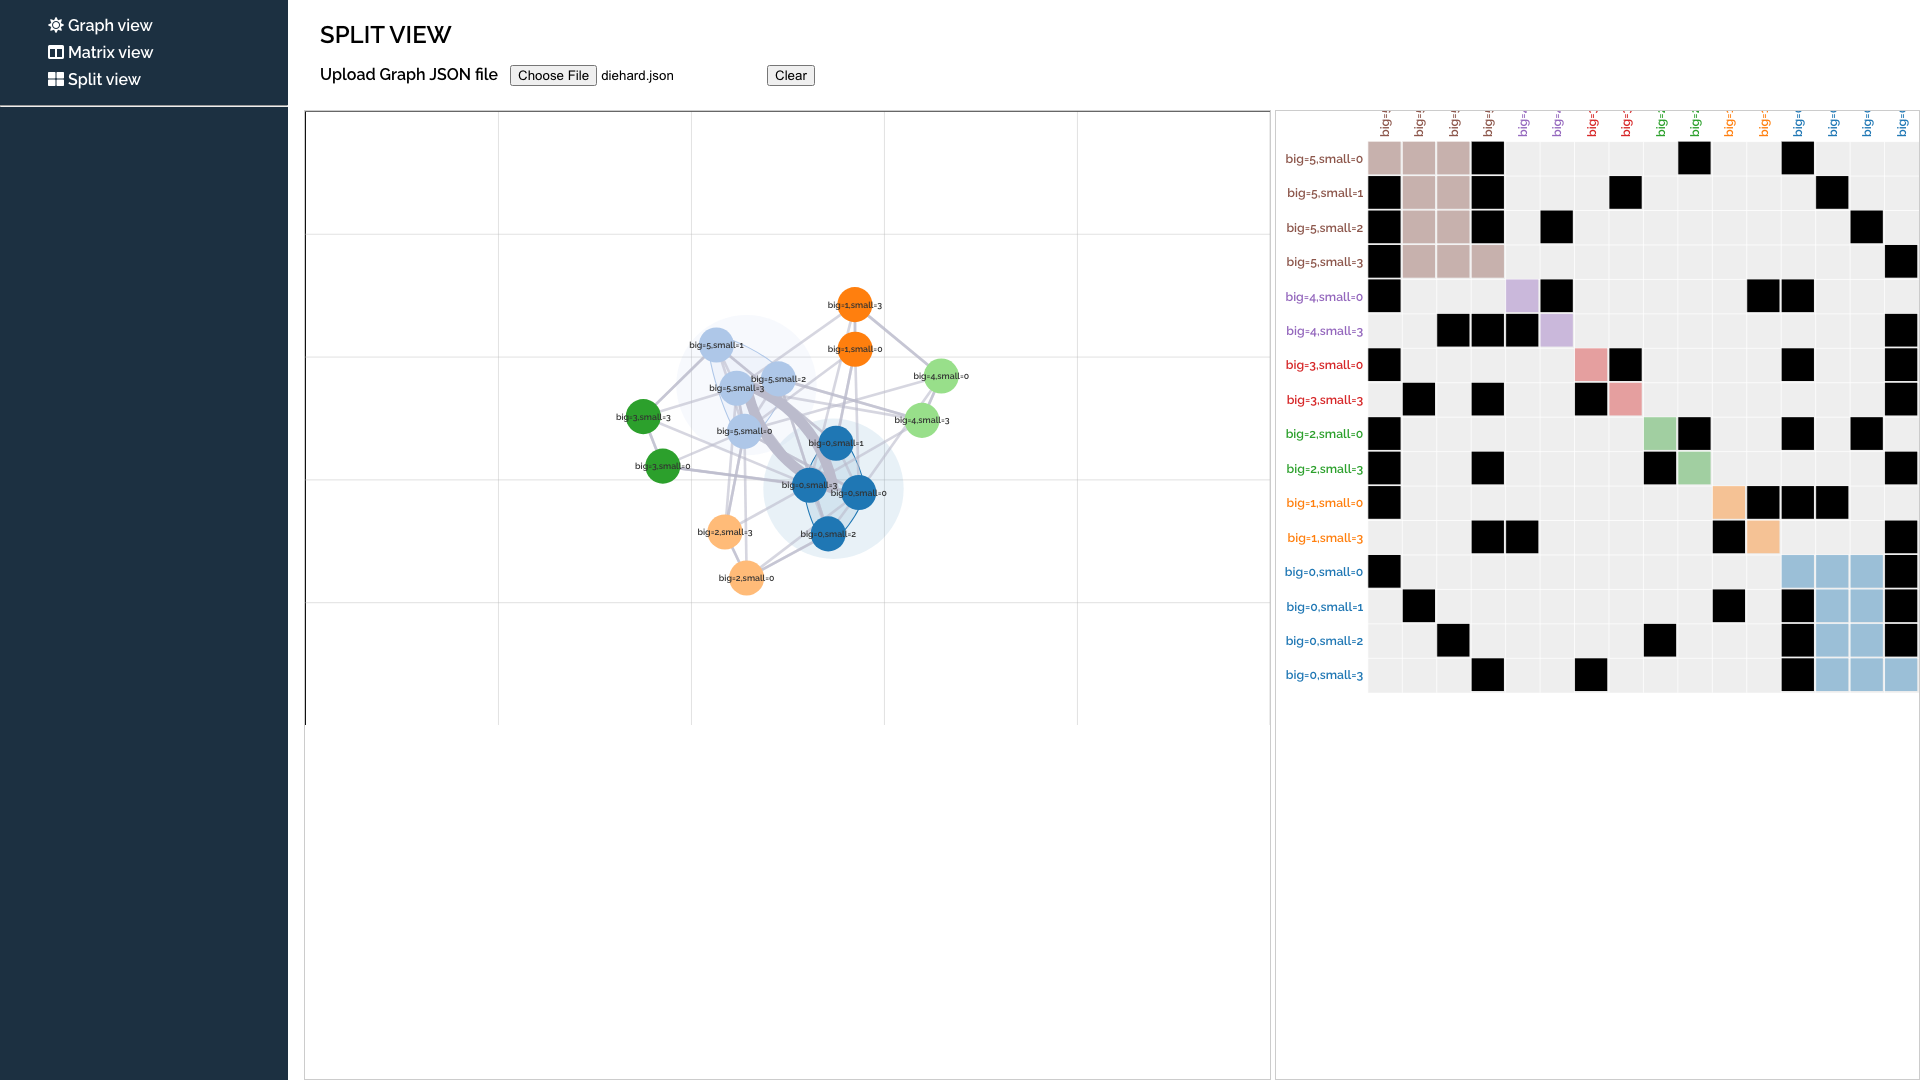
\includegraphics[width=\textwidth]{figures/diehard_split.png}
\caption{The coordinated split view showing the Die Hard water jugs specification. Left: clustered force-directed graph with six clusters (one per big-jug value), color-coded by cluster membership, with convex hulls around clusters with three or more members. Right: adjacency matrix with cluster-based ordering, showing transitions as filled cells and cluster boundaries as colored blocks along the diagonal.}
\label{fig:diehard_split}
\end{figure*}

\subsection{Clustered Force-Directed Graph View}

The graph view (Fig.~\ref{fig:diehard_split}, left) renders the state space as a clustered force-directed layout built with D3.js v4. The design addresses challenge D1 (mismatch between topology and semantics) by incorporating cluster-aware forces into the layout algorithm.

\textbf{Layout algorithm.} The layout uses D3's force simulation with five forces: (1) a centering force that keeps the graph centered in the viewport, (2) a charge force that repels nodes from each other to prevent overlaps, (3) a collision detection force that enforces a minimum distance between nodes, (4) a cluster attraction force that pulls nodes toward the centroid of their cluster, and (5) a link force that constrains connected nodes to a target distance. The cluster attraction force is the key addition: for each node, it computes the centroid of all nodes in the same cluster and applies a force pulling the node toward that centroid. The strength and distances of these forces were tuned through iterative experimentation to produce stable, readable layouts.

\textbf{Visual encoding.} Nodes are rendered as circles colored by cluster membership using D3's categorical color scale. Each node displays a text label showing its state description (e.g., \texttt{big=3,small=0}). Edges are rendered as lines connecting source and target nodes, with arrowheads indicating direction. Convex hulls are drawn around clusters with three or more members using a semi-transparent fill of the cluster color, providing a visual boundary that reinforces the cluster grouping.

\textbf{Interaction.} Hovering over a node triggers a detail-on-demand interaction: the selected node and its immediate neighbors (connected by incoming or outgoing edges) remain at full opacity, while all other nodes fade to 20\% opacity. Connected edges turn red; unconnected edges fade. A tooltip displays the state label, cluster identifier, and in/out degree. This dimming interaction directly supports task T3 (transition inspection) by isolating the selected state's connectivity from the visual clutter of the full graph. When the user moves the mouse away from the node, the full graph is restored.

\textbf{Cluster-level aggregation.} For clusters with more than two members, a centroid circle is drawn at the cluster center, providing a visual anchor for the cluster. This centroid can serve as a reference point when examining inter-cluster connectivity and helps engineers maintain orientation in the graph layout.

\subsection{Adjacency Matrix View}

The matrix view (Fig.~\ref{fig:diehard_split}, right) renders the state-transition graph as an adjacency matrix built with D3.js v5. This view addresses challenge D2 (visual clutter from dense connectivity) by providing a representation where every possible connection has a dedicated cell, eliminating edge crossings entirely.

\textbf{Layout.} The matrix is constructed as a grid of rectangular cells, with rows and columns corresponding to states. The matrix is ordered by cluster membership (default), which groups states belonging to the same cluster together along the diagonal. Within each cluster, states are ordered by node identifier. This ordering ensures that intra-cluster transitions appear as dense blocks along the diagonal, while inter-cluster transitions form off-diagonal patterns. The matrix also supports reordering by node identifier, which provides a sequential view of the state space.

\textbf{Visual encoding.} A filled (black) cell at position $(i, j)$ indicates a transition from state $i$ to state $j$. Cells within the same cluster (where the row state and column state share the same cluster identifier) are lightly shaded with the cluster color at 40\% opacity, making cluster boundaries immediately visible as colored blocks along the diagonal. Row and column labels display the state description (label or identifier) and are colored by cluster membership.

\textbf{Interaction.} Hovering over a row or column label highlights that state's entire row and column, with connected cells (cells where a transition exists) outlined in red. A tooltip displays the state label and cluster identifier. Hovering over a filled cell displays a tooltip showing the source state, target state, and action name (if available) for the transition. This interaction supports task T3 (transition inspection) by providing precise information about individual transitions.

\textbf{Reordering.} A dropdown control allows the user to switch between cluster-based ordering and node-identifier ordering. Cluster ordering reveals structural patterns related to the specification's variable groupings, while node-identifier ordering provides a sequential view that may be useful for tracing paths through the state space.

\subsection{Coordinated Split View}

The split view (Fig.~\ref{fig:diehard_split}) displays the graph and matrix views side by side in a 3:2 width ratio, with the graph view occupying the larger portion (reflecting its higher spatial requirements) and the matrix view occupying the smaller portion. This view addresses challenge D3 (task diversity) by enabling engineers to use both representations simultaneously and cross-reference between them.

\textbf{Architecture.} Both views are embedded as iframes within the split view page. An \texttt{embedded} query parameter is passed to each iframe, which triggers CSS rules that hide the navigation bar and toolbar in the embedded views, maximizing the space available for the visualization. The parent page provides a shared toolbar with file upload and clear controls that forward data to both iframes.

\textbf{Coordination protocol.} The bidirectional highlighting is implemented through the \texttt{postMessage} API. When a user hovers over a node in the graph view, the graph view sends a \texttt{highlight} message containing the node identifier to its parent window. The parent window forwards this message to the matrix view, which responds by highlighting the corresponding row and column headers in red and outlining connected cells. The reverse interaction also works: hovering over a label or cell in the matrix sends a \texttt{highlight} message that is forwarded to the graph view, which highlights the corresponding node and dims non-connected nodes. When the user moves the mouse away, an \texttt{unhighlight} message restores both views to their default state.

\textbf{Cross-referencing workflow.} This coordination supports a powerful cross-referencing workflow. An engineer can identify an interesting cluster in the matrix (by observing a dense block of transitions along the diagonal) and then hover over a state in that block to immediately locate it spatially in the graph view. Conversely, the engineer can select a node in the graph view and examine its complete connectivity pattern---all incoming and outgoing transitions---in the matrix view, where the pattern is visible as a highlighted row and column without the visual clutter of overlapping edges. This bidirectional cross-referencing directly supports tasks T3 (transition inspection) and T4 (path tracing) by enabling engineers to combine spatial intuition from the graph with precise structural information from the matrix.

%% ============================================================
\section{Usage Scenarios}
\label{sec:scenarios}

We demonstrate our tool on three TLA+ specifications drawn from the formal methods literature, each illustrating different aspects of the multi-view approach. Following the design study methodology~\cite{sedlmair2012design}, we present detailed usage scenarios that show how the tool supports the tasks identified in our task analysis. The specifications range from a simple cyclic system (12 states, 12 transitions) to a moderately complex combinatorial system (16 states, 58 transitions), representing the range of state-space sizes most commonly encountered in visual exploration of TLA+ specifications.

\begin{figure}[t]
\centering
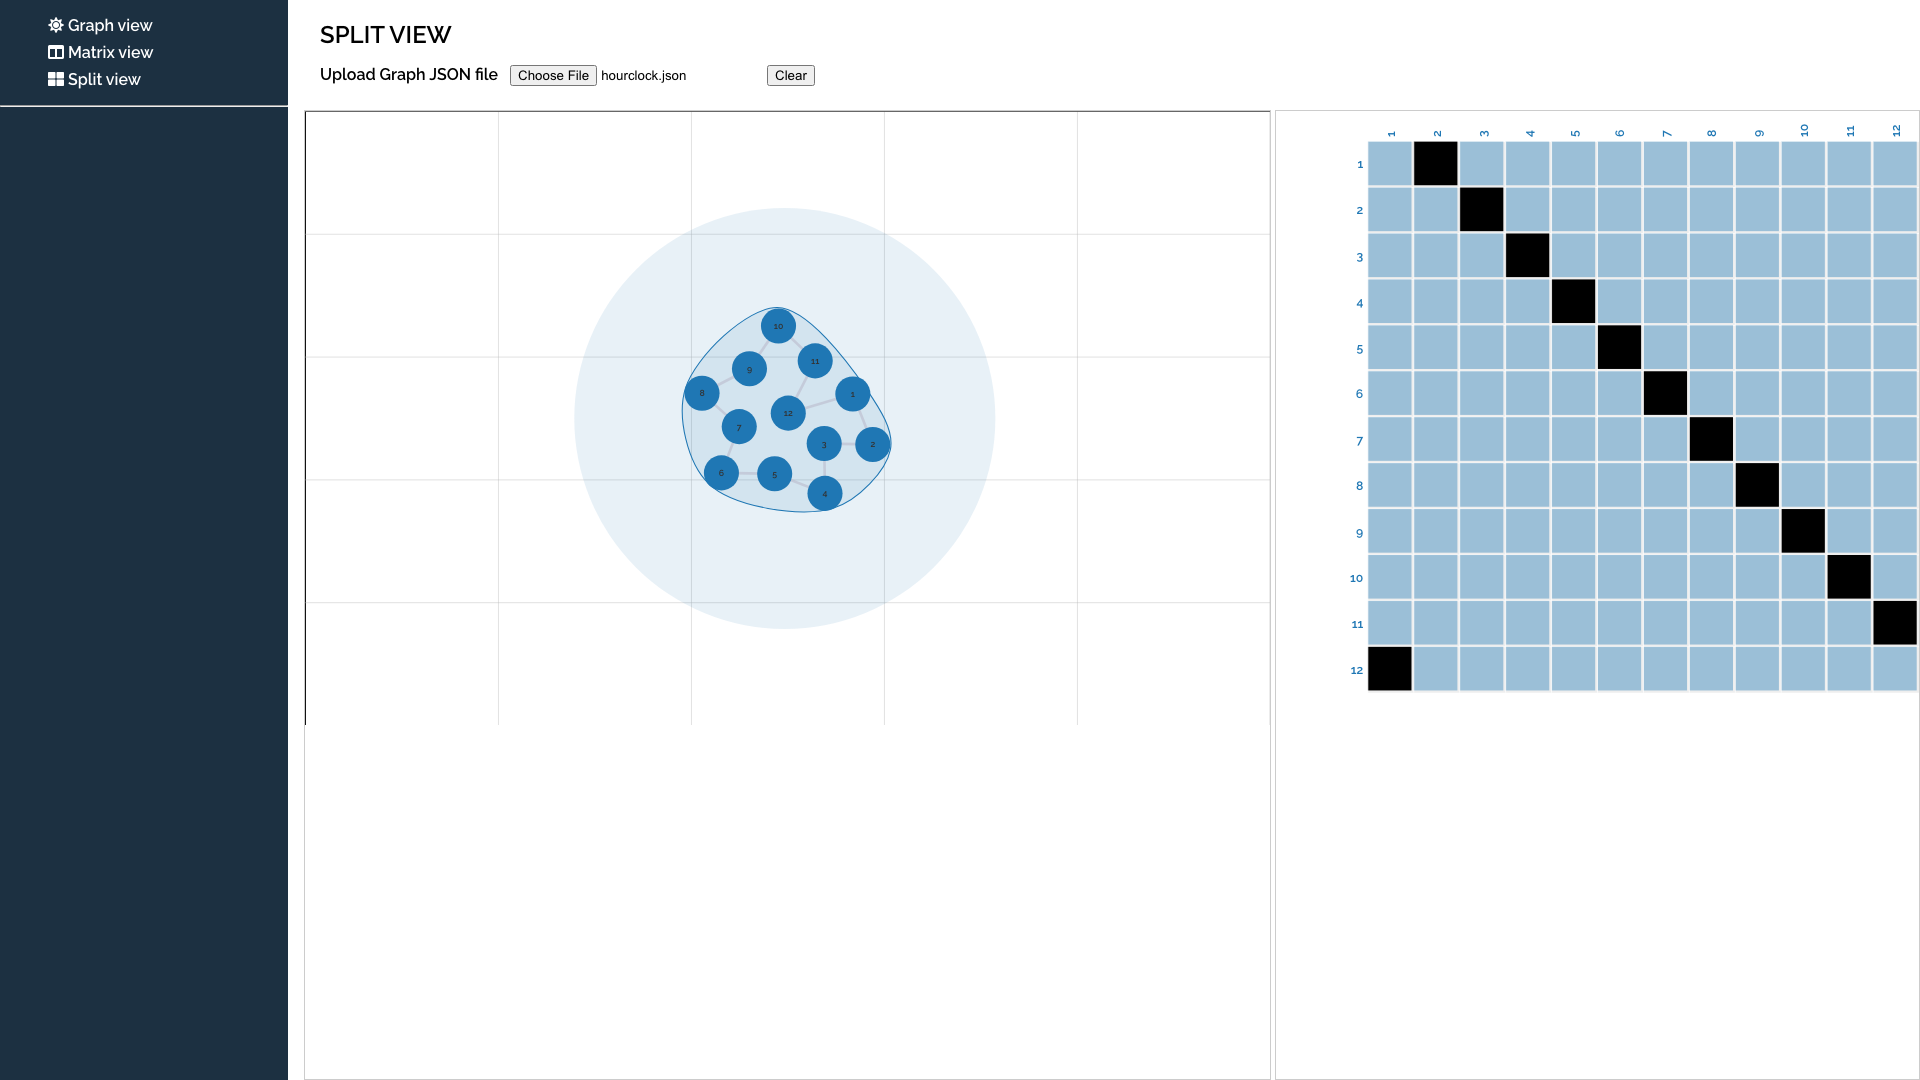
\includegraphics[width=\columnwidth]{figures/hourclock_split.png}
\caption{The coordinated split view for the HourClock specification. Left: 12 nodes in a single cluster arranged by force-directed layout. Right: adjacency matrix showing the cyclic pattern as a diagonal band one step above the main diagonal.}
\label{fig:hourclock_split}
\end{figure}

\subsection{HourClock: Simple Cyclic Behavior}

The HourClock specification~\cite{lamport2003specifying} is a canonical example from the TLA+ literature that models a clock cycling through values 1 to 12 via a single action \texttt{HCnxt}. The state space consists of 12 states, all belonging to a single cluster (since there is only one variable, \texttt{hr}), connected in a cycle where each state transitions to the next hour value, with state 12 wrapping back to state 1.

\textbf{Graph view (T1, T2).} The graph view (Fig.~\ref{fig:hourclock_split}, left) displays all 12 nodes in a single cluster, drawn within a convex hull. The cyclic structure is visually apparent: nodes are arranged roughly in a circle by the force-directed layout, with edges connecting consecutive states. However, the exact ordering of states around the circle depends on the force simulation's convergence and is not guaranteed to reflect the logical sequence 1--12. The engineer can observe that all states belong to a single cluster (T2) and that the graph has a regular, ring-like structure (T1), but verifying the exact cyclic ordering requires inspecting individual edges.

\textbf{Matrix view (T1, T3).} The matrix view (Fig.~\ref{fig:hourclock_split}, right) reveals the cyclic structure with much greater clarity. With states ordered by node identifier, the matrix shows a distinctive pattern: a diagonal band of filled cells one step above the main diagonal, plus a single cell at position $(12, 1)$ representing the wrap-around transition from hour 12 back to hour 1. This pattern is immediately recognizable as a cycle: exactly one outgoing transition per state, exactly one incoming transition per state, and no other connections. An engineer can verify at a glance that the specification is deterministic (one outgoing transition per state) and complete (every state has a successor).

\textbf{Coordinated view (T3).} In the split view, the engineer can hover over a specific state in the graph (e.g., state \texttt{hr=6}) and immediately see the corresponding row and column highlighted in the matrix, confirming that state 6 has exactly one incoming transition (from state 5) and one outgoing transition (to state 7). This cross-referencing is straightforward for this simple specification but demonstrates the interaction protocol that becomes essential for more complex state spaces.

\textbf{Insight.} For this regular, single-cluster specification, the matrix view is more informative than the graph view. The matrix unambiguously reveals the specification's structure---a deterministic cycle---while the graph view requires manual tracing of edges to confirm the same property. This observation supports the finding of Ghoniem et al.~\cite{ghoniem2004comparison} that matrix representations are superior for tasks involving precise connectivity assessment.

\begin{figure}[t]
\centering
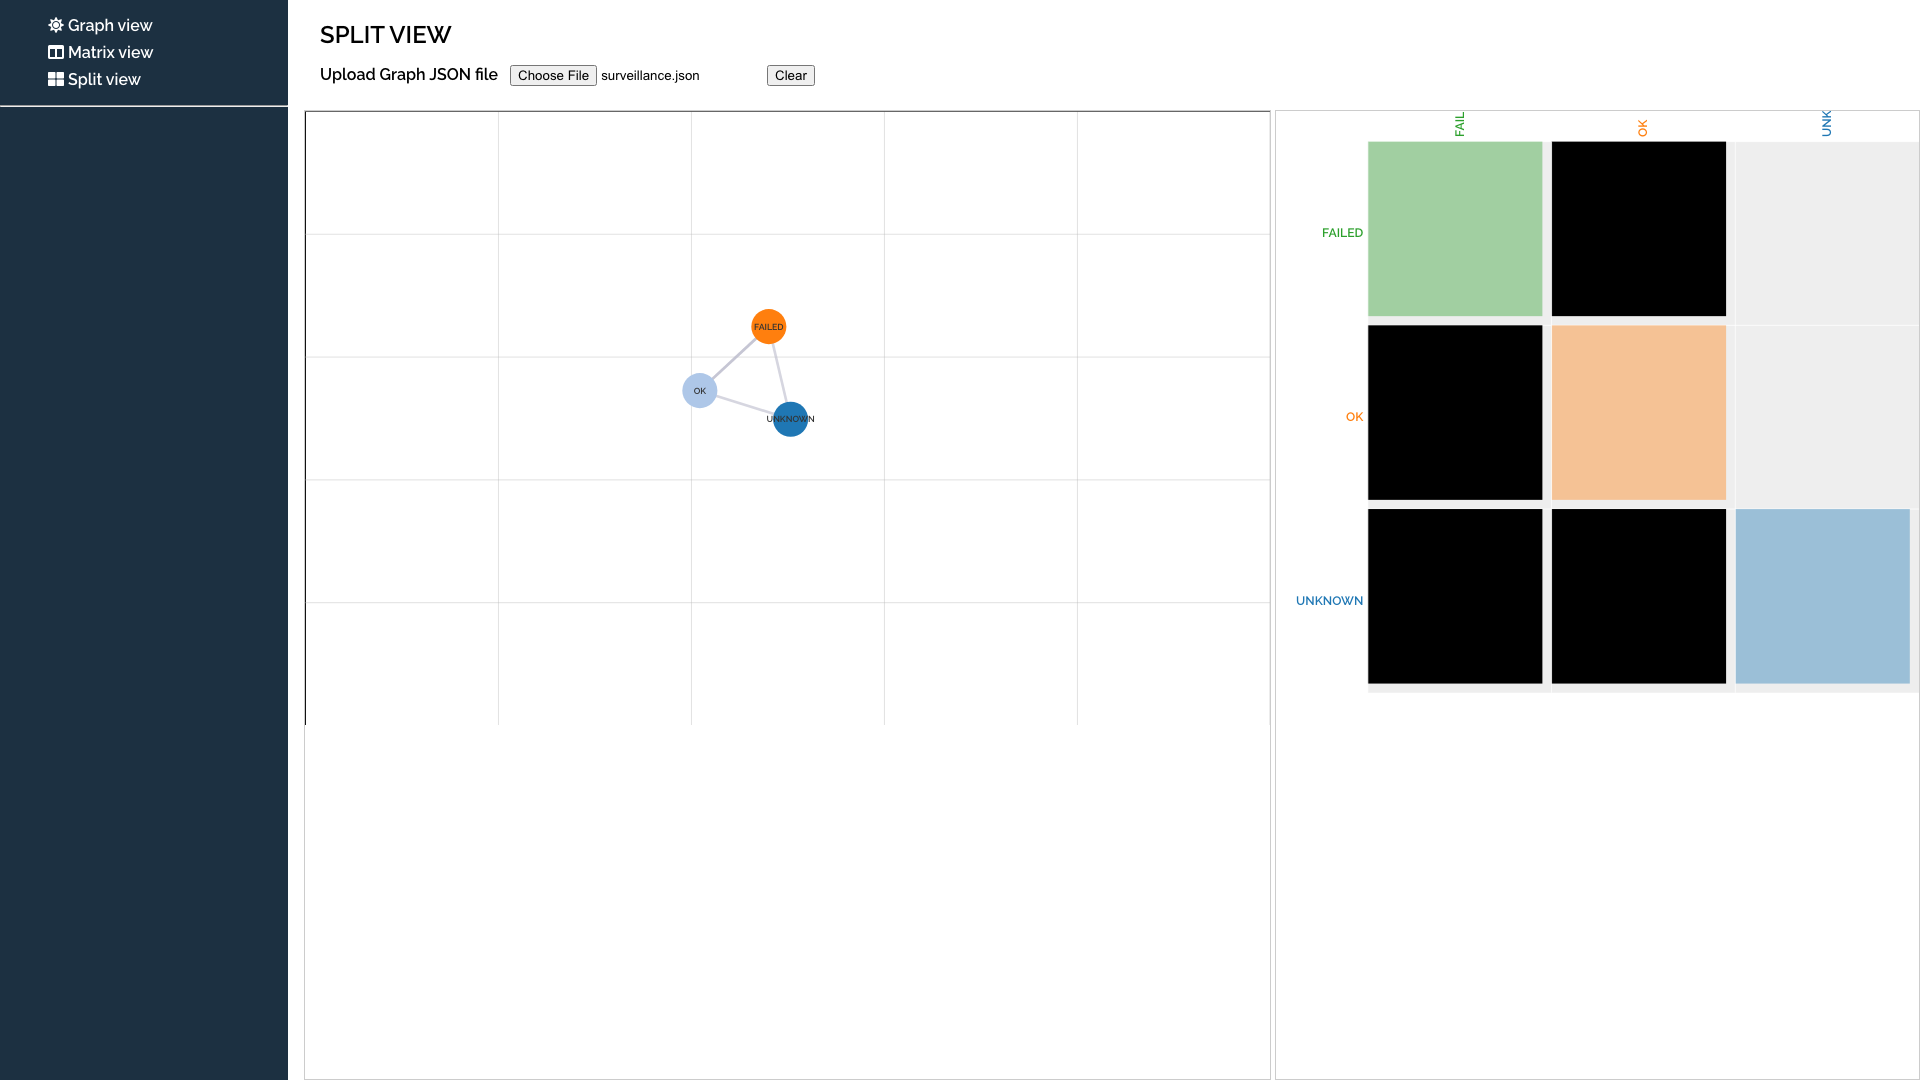
\includegraphics[width=\columnwidth]{figures/surveillance_split.png}
\caption{The coordinated split view for the Surveillance System specification. Left: three nodes (UNKNOWN, OK, FAILED) each in a distinct cluster. Right: $3 \times 3$ adjacency matrix showing four transitions with action names visible via tooltips.}
\label{fig:surveillance_split}
\end{figure}

\subsection{Surveillance System: Multi-State with Labeled Transitions}

The surveillance system specification models a simplified and obfuscated version of a distributed surveillance system derived from a large industry project built from a number of distributed sensors. This is a challenging system to both understand and debug due to the event-based and asynchronous nature of the code implementing the system. At any given time, the system should be in one state: Unknown, Running (OK), or Failed. When the surveillance system starts, it initially goes to the Unknown state. It then waits for messages from one of the sensors for 10 seconds. If a message is received during this time, it goes to the Running state; otherwise, if nothing happens, it goes to the Failed state. The system can alternate between the Running and Failed states: if no message is received in a ten-second window it goes to Failed, and it goes back to Running when a message is received. Fig.~\ref{fig:surveillance_spec} shows the TLA+ specification.

\begin{figure}[t]
\begin{lstlisting}[language={},morekeywords={EXTENDS,CONSTANTS,VARIABLES,Init,Next}]
EXTENDS Naturals
CONSTANTS UNKNOWN, OK, FAILED

VARIABLES state

report_received ==
    /\ state' = OK

timeout ==
    /\ state' = FAILED

Init ==
    /\ state = UNKNOWN

Next ==
    \/ report_received
    \/ timeout
\end{lstlisting}
\caption{Simplified TLA+ specification of the Surveillance System. The single variable \texttt{state} can hold values UNKNOWN, OK, or FAILED, with two actions defining the transitions.}
\label{fig:surveillance_spec}
\end{figure}

The state space consists of 3 states, each in its own cluster (since the only variable is \texttt{state}, and each state has a unique value), connected by 4 transitions.

\textbf{Graph view (T1, T2, T3).} The graph view (Fig.~\ref{fig:surveillance_split}, left) displays three labeled nodes---\textit{UNKNOWN}, \textit{OK}, and \textit{FAILED}---with directed edges between them. The visualization resembles a traditional state machine diagram, which is appropriate for this small specification. Each node is colored differently (since each belongs to a different cluster), and the labels are directly visible on the nodes. The spatial layout clearly shows that \textit{UNKNOWN} is the initial state (no incoming transitions from the initial set), \textit{OK} and \textit{FAILED} are reachable from \textit{UNKNOWN}, and \textit{OK} and \textit{FAILED} can transition to each other. Engineers familiar with state machine notation can read this visualization immediately.

\textbf{Matrix view (T3).} The matrix view (Fig.~\ref{fig:surveillance_split}, right) shows a $3 \times 3$ grid with four filled cells corresponding to the four transitions. The matrix provides a compact summary of the complete transition function: by scanning the row for \textit{UNKNOWN}, the engineer can see that it has outgoing transitions to \textit{OK} and \textit{FAILED}. Hovering over a filled cell displays a tooltip showing the action name: the transition from \textit{UNKNOWN} to \textit{OK} is triggered by \texttt{report\_received}, while the transition from \textit{UNKNOWN} to \textit{FAILED} is triggered by \texttt{timeout}. This action-level detail supports task T3 (transition inspection) without requiring the engineer to refer back to the specification text.

\textbf{Coordinated view (T3, T4).} The coordinated highlighting reveals the full connectivity of each state. Selecting the \textit{FAILED} node in the graph highlights its row and column in the matrix, immediately revealing three pieces of information: (1) \textit{FAILED} can be reached from \textit{UNKNOWN} via \texttt{timeout} and from \textit{OK} via \texttt{timeout}; (2) \textit{FAILED} can transition to \textit{OK} via \texttt{report\_received}; and (3) \textit{FAILED} has no self-loop (the diagonal cell is empty). This integrated view enables the engineer to verify the specification's behavior: the system can recover from a \textit{FAILED} state when a sensor report is received, which matches the intended design.

\textbf{Insight.} For this small, multi-cluster specification with labeled transitions, the graph view provides the most intuitive overview, as the spatial layout directly corresponds to the mental model of a state machine. However, the matrix view's ability to show action names via tooltips provides valuable detail that complements the spatial overview. The coordinated view enables efficient verification of the specification by combining spatial intuition with precise connectivity information.

\subsection{Die Hard Water Jugs: State Explosion and Clustering}

The Die Hard water jugs problem is a well-known combinatorial puzzle (featured in the film \textit{Die Hard with a Vengeance}) that models two water jugs with capacities of 5 gallons (\texttt{big}) and 3 gallons (\texttt{small}). The specification defines two variables and six possible actions: \texttt{FillBig} (fill the big jug to capacity), \texttt{FillSmall} (fill the small jug), \texttt{EmptyBig} (empty the big jug), \texttt{EmptySmall} (empty the small jug), \texttt{BigToSmall} (pour from big to small until small is full or big is empty), and \texttt{SmallToBig} (pour from small to big). Each state is defined by the pair of values $(\mathtt{big}, \mathtt{small})$, representing the current water level in each jug. The goal is to reach the state $\mathtt{big}=4, \mathtt{small}=0$.

The TLC model checker enumerates 16 reachable states and 58 transitions for this specification---already dense enough to produce significant visual clutter in a flat node-link diagram. This specification is particularly interesting for visualization because it exhibits the state explosion phenomenon at a scale that is still amenable to visual exploration: with only two variables, the state space is comprehensible in principle, but the density of transitions (an average of 3.6 outgoing transitions per state) makes a flat node-link diagram illegible. States are grouped by the value of the \texttt{big} variable into six clusters: \texttt{big=0} (4 states), \texttt{big=1} (2 states), \texttt{big=2} (2 states), \texttt{big=3} (2 states), \texttt{big=4} (2 states), and \texttt{big=5} (4 states).

\textbf{Graph view (T1, T2).} The clustered force-directed layout spatially separates the six clusters, with each cluster rendered in a distinct color. Clusters with three or more members (\texttt{big=0} and \texttt{big=5}) are enclosed in convex hulls, providing clear visual boundaries. The engineer can immediately observe (T1) that the state space has a non-trivial structure with multiple clusters of varying sizes, and (T2) identify which clusters correspond to which big-jug values. The two largest clusters (big=0 and big=5) are at opposite ends of the variable's range, each containing states where the small jug holds different amounts of water. The spatial separation of clusters makes it easy to see that inter-cluster transitions (which change the big-jug value) dominate the visualization, as dense bundles of edges connect the clusters.

\textbf{Comparison with unclustered layout.} Rendering this specification as a flat force-directed layout without clustering (Fig.~\ref{fig:hairball}) produces an illegible tangle of overlapping nodes and edges where no meaningful structure is visible. With 16 nodes and 58 edges, edge crossings obscure all cluster structure and make it impossible to trace individual transitions. Our clustered multi-view approach transforms the same data into a readable visualization where cluster membership, cluster sizes, and inter-cluster connectivity patterns are all visible.

\textbf{Matrix view (T1, T2, T3).} The adjacency matrix, ordered by cluster membership, reveals a rich block structure. Intra-cluster transitions appear as dense blocks along the diagonal---for example, the \texttt{big=0} cluster (4 states) forms a $4 \times 4$ block in the upper-left corner with several filled cells representing transitions between states that share the same big-jug value but differ in small-jug value. Inter-cluster transitions form off-diagonal patterns that reveal the connectivity between clusters.

The matrix makes several structural properties immediately visible that would be difficult to discern in the graph view: (1) every state has exactly four outgoing transitions (four filled cells per row), reflecting the six actions minus those that are disabled in certain states; (2) the transition pattern is not symmetric---the matrix is not symmetric about the diagonal, reflecting the directed nature of the state transitions; (3) certain cluster pairs have dense connectivity (e.g., transitions between \texttt{big=0} and \texttt{big=5} are common because \texttt{FillBig} from any state with \texttt{big=0} reaches \texttt{big=5}), while others have sparse or no connectivity.

\textbf{Coordinated view (T3, T4).} The coordinated view enables the most powerful analysis of this complex specification. Consider an engineer investigating how to reach the goal state \texttt{big=4,small=0}---the solution to the Die Hard puzzle. The engineer can locate this state in the graph view (in the \texttt{big=4} cluster) and hover over it, causing the matrix view to highlight the corresponding row and column. The column highlighting reveals all states that have a transition \textit{to} the goal state (incoming transitions), while the row highlighting reveals all states reachable \textit{from} the goal state (outgoing transitions).

By examining the highlighted column in the matrix, the engineer discovers which predecessor states can reach the goal. The engineer can then hover over each predecessor in the matrix to trace the path backward through the state space, building a mental model of the solution path. At each step, the graph view provides spatial context---showing where each state sits relative to its cluster---while the matrix view provides precise connectivity information. This interleaved exploration, alternating between views, directly supports task T4 (path tracing) and demonstrates the value of coordinated views for complex specifications.

\textbf{Insight.} For this complex specification with 16 states and 58 transitions, neither the graph view nor the matrix view alone provides a complete understanding. The graph view excels at showing cluster structure and spatial relationships (T1, T2) but becomes cluttered when examining individual transitions (T3). The matrix view excels at showing precise connectivity patterns and transition counts (T3) but lacks the spatial intuition of the graph. The coordinated split view combines both strengths, enabling engineers to navigate the state space effectively by cross-referencing between representations. This observation validates our design decision to provide a multi-view approach rather than optimizing a single representation.

%% ============================================================
\section{Discussion}
\label{sec:discussion}

Our tool demonstrates that coordinated multi-view visualization with semantic clustering substantially improves the comprehension of TLA+ state spaces compared to a single-view force-directed layout. In this section, we reflect on our design decisions, discuss preliminary usage experience, analyze scalability, and identify limitations.

\subsection{Reflection on Design Decisions}

Our design process confirmed several findings from the visualization literature. First, the complementary strengths of graph and matrix representations~\cite{ghoniem2004comparison, henry2006matrixexplorer} are clearly evident in our usage scenarios: the graph view provides spatial intuition about cluster structure, while the matrix view reveals precise connectivity patterns. The HourClock scenario demonstrated that the matrix view can be strictly more informative than the graph view for regular specifications, while the Die Hard scenario demonstrated that neither view alone is sufficient for complex specifications.

Second, the use of variable-based clustering proved highly effective for TLA+ state spaces. Unlike general graphs where community detection algorithms must infer structure from topology, TLA+ specifications provide semantically meaningful groupings through their variable definitions. This domain-specific insight---that states sharing variable values form meaningful clusters---is analogous to the insight of Wongsuphasawat et al.~\cite{wongsuphasawat2018tensorflow} that TensorFlow operations sharing namespace prefixes form meaningful groups. In both cases, domain knowledge provides a clustering criterion that is more meaningful than purely topological approaches.

Third, the bidirectional brushing-and-linking interaction proved essential for complex specifications. The Die Hard scenario demonstrated that alternating between views---using the graph for spatial orientation and the matrix for precise connectivity---enables a form of exploration that neither view supports alone. This finding is consistent with the principles of coordinated multiple views articulated by Roberts~\cite{roberts2007cmv} and the guidelines of Wang Baldonado et al.~\cite{baldonado2000guidelines}.

\subsection{Preliminary Usage Experience}

The multi-view tool described in this paper has been developed iteratively in the context of industry projects that employ TLA+-based event model specifications. Engineers in these projects who previously struggled to understand the TLA+ domain-specific language reported that visualization of state spaces greatly assisted their understanding and use of the specifications. Feedback from these engineers indicated that force-directed layouts became unreadable for specifications with more than approximately 20 states, directly motivating the multi-view approach presented in this paper.

However, we have not yet conducted a formal user evaluation of the multi-view tool itself. The usage scenarios presented in Section~\ref{sec:scenarios} are based on our own expert analysis rather than observed user behavior. A formal evaluation is a priority for future work, as discussed below.

\subsection{Scalability Analysis}

Our tool targets TLA+ specifications with tens to low hundreds of states, which represents the most common range for visual exploration. Within this range, we observe the following scalability characteristics:

\textbf{Graph view.} The clustered force-directed layout performs well for specifications with up to approximately 50 states. Beyond this, the layout becomes increasingly cluttered, even with clustering, due to the density of inter-cluster edges. The force simulation's convergence time also increases with the number of nodes, potentially causing visible oscillation during initial rendering. For specifications with more than 100 states, the graph view provides a useful overview but becomes difficult to use for detailed inspection.

\textbf{Matrix view.} The adjacency matrix scales better than the graph view, as the grid layout eliminates edge crossings regardless of graph density. However, the matrix size grows quadratically with the number of states ($n \times n$ cells for $n$ states), and label readability decreases as the cell size shrinks. For specifications with more than approximately 100 states, the matrix cells become too small to interact with effectively, and the labels become illegible without zooming.

\textbf{Coordinated view.} The coordinated interaction adds negligible overhead, as the \texttt{postMessage} communication involves only small JSON objects. The rendering performance is dominated by the individual view performance, and the split view layout allocates screen space efficiently through the 3:2 ratio.

\subsection{Limitations and Future Work}

We identify several limitations and directions for future work.

\textbf{Scalability beyond hundreds of states.} While our approach handles specifications with tens to low hundreds of states effectively, very large specifications (thousands of states) require additional techniques. We plan to investigate hierarchical clustering with expandable sub-clusters, following the approach of the TensorFlow Graph Visualizer~\cite{wongsuphasawat2018tensorflow}, as well as abstract state grouping supported natively by TLA+. Semantic zooming, where the level of detail adapts to the zoom level, could enable the matrix view to scale to larger specifications by showing cluster-level summaries at low zoom and individual cells at high zoom.

\textbf{Integration with TLC.} Currently, the JSON state graph must be manually generated from TLC model checker output through a transformation script. Direct integration with the TLA+ Toolbox would streamline the workflow, allowing engineers to visualize the state space immediately after model checking completes. Live re-visualization as specifications evolve would further tighten the feedback loop between specification writing and visual inspection.

\textbf{User evaluation.} A rigorous evaluation of the multi-view tool is our highest priority for future work. We plan to pursue this along two complementary tracks. First, following the qualitative feedback approach of Wongsuphasawat et al.~\cite{wongsuphasawat2018tensorflow}, we plan to deploy the tool to engineers working with TLA+ specifications in industry projects and gather feedback through structured questionnaires, direct observation of usage, and collection of usage patterns ``in the wild.'' Second, we plan to conduct a controlled user study comparing task performance across the three views (graph only, matrix only, coordinated split) for each of the four tasks (T1--T4) across specifications of varying complexity. Such a study should measure task completion time, accuracy, and user satisfaction, providing quantitative evidence for the effectiveness of the multi-view approach compared to single-view alternatives.

\textbf{Bidirectional editing.} Supporting edits from the visualization back to the specification would close the loop between visual debugging and specification refinement. An engineer who identifies a missing transition in the matrix view could click to add it, with the change propagated back to the TLA+ source. This capability would transform the tool from a read-only inspector to an interactive development environment.

\textbf{Edge bundling.} Hierarchical edge bundling~\cite{holten2006hierarchical} could significantly reduce visual clutter in the graph view for specifications with dense inter-cluster connectivity. By routing edges along the cluster hierarchy, edge bundling would preserve the readability of the clustered layout while showing aggregate connectivity patterns between clusters.

\textbf{Temporal exploration.} TLA+ specifications describe temporal behavior, but our current tool shows only the static state graph. Animating transitions along execution traces---highlighting the current state and advancing through a sequence of actions---would support a more dynamic form of exploration. Stepping functionality that allows engineers to advance through states one action at a time would be a natural extension of the multi-view context.

\textbf{Additional matrix ordering.} Beyond cluster-based and identifier-based ordering, additional matrix reordering algorithms~\cite{behrisch2016reordering} could reveal different structural patterns. For example, reverse Cuthill-McKee ordering could minimize the bandwidth of the matrix, concentrating transitions near the diagonal and making sequential patterns more visible.

%% ============================================================
\section{Conclusion}
\label{sec:conclusion}

We presented a design study of a web-based multi-view visualization tool for TLA+ state spaces that combines a clustered force-directed graph, an adjacency matrix with cluster-based ordering, and a coordinated split view with bidirectional brushing-and-linking. Our design was informed by a task analysis identifying four key engineering tasks (overview, cluster identification, transition inspection, and path tracing), a characterization of the data properties of TLC model checker output, and an iterative design process that explored and evaluated three visualization approaches.

Through detailed usage scenarios on three TLA+ specifications of increasing complexity, we demonstrated how the complementary strengths of graph and matrix representations support different analysis tasks. The graph view provides spatial intuition about cluster structure and inter-cluster connectivity; the matrix view reveals precise connectivity patterns at higher information density without the visual clutter of edge crossings; and the coordinated split view enables cross-referencing between representations, supporting a form of exploration that neither view achieves alone.

Our tool addresses a practical need in the formal methods community: as TLA+ adoption grows in industry~\cite{newcombe2015amazon, resch2017tla}, engineers who are not formal methods experts need visual tools to comprehend the state spaces produced by model checking. By adapting techniques from the graph visualization and coordinated multiple views literature to the specific structure of TLA+ state spaces, our tool makes formal specifications more accessible and supports the verification workflow that is critical for mission-critical systems engineering.

The source code and example datasets are available as a web application that runs entirely in the browser, requiring no installation beyond uploading a JSON file derived from TLC model checker output. We believe this low barrier to entry, combined with the multi-view visualization approach, represents a meaningful step toward making formal methods tools more usable for a broader engineering audience.

\balance

\bibliographystyle{IEEEtran}
\bibliography{references}

\end{document}


